\section{Mathieu函数}
\subsection{一般形式}
Mathieu方程形如
\begin{equation*}
	\frac{\d^2 y}{\d z^2} + (\lambda - 2q \cos(2z)) y = 0.
\end{equation*}
展开为Floquent解
\begin{equation*}
	y(z) = \sum_{k=-\infty}^{\infty} c_k e^{i(\nu + 2k)z}
\end{equation*}

代入得临项系数递推关系
\begin{equation*}
	c_{k+1} - \frac{D_k}{q} c_k + c_{k-1} = 0, \quad D_k = \lambda - (\nu + 2k)^2.
\end{equation*}

写成无穷连分式，即
\begin{equation*}
	\frac{c_k}{c_{k-1}} = \frac{q}{D_k - \dfrac{q^2}{D_{k+1} - \dfrac{q^2}{D_{k+2} - \dots}}}, \quad \frac{c_{k-1}}{c_k} = \frac{q}{D_{k-1} - \dfrac{q^2}{D_{k-2} - \dfrac{q^2}{D_{k-3} - \dots}}}.
\end{equation*}
\begin{equation*}
	D_k - \frac{q^2}{D_{k+1} - \dfrac{q^2}{D_{k+2} - \dots}} = \frac{q^2}{D_{k-1} - \dfrac{q^2}{D_{k-2} - \dfrac{q^2}{D_{k-3} - \dots}}}.
\end{equation*}
\begin{equation*}
	\lambda - (\nu + 2k)^2 - \frac{q^2}{\lambda - (\nu + 2k + 2)^2 - \dfrac{q^2}{\lambda - (\nu + 2k + 4)^2 - \dots}} = \frac{q^2}{\lambda - (\nu + 2k - 2)^2 - \dfrac{q^2}{\lambda - (\nu + 2k - 4)^2 - \dots}}.
\end{equation*}

对 \(\nu = 2n\)（\(n \in \mathbb{N}\)）的全周期解：

若 \(c_{-n}\) 有限，由 \(\left( \dfrac{c_{-n}}{c_{-n-1}} \right) \left( \dfrac{c_{-n-1}}{c_{-n}} \right) = 1\) 得
\begin{align*}
	 & \lambda - 4 - \frac{2q^2}{\lambda} = \frac{q^2}{\lambda - 16 - \dfrac{q^2}{\lambda - 36 - \dots}}                                                                                                       \\
	 & \implies \lambda - (2n)^2 - \frac{q^2}{\lambda - (2n - 2)^2 - \dots - \dfrac{q^2}{\lambda - 4 - \dfrac{2q^2}{\lambda}}} = \frac{q^2}{\lambda - (2n + 2)^2 - \dfrac{q^2}{\lambda - (2n + 4)^2 - \dots}}.
\end{align*}
该式解记为 \(\lambda = a_{2n}(q)\)，对应系数满足 \(c_{-n-l} = c_{-n+l}\)（\(l \in \mathbb{N}\)），进而
\begin{equation*}
	y = \mathrm{ce}_{2n}(z) = \sum_{s=-\infty}^{\infty} c_{s-n} e^{2isz} = c_{-n} + 2 \sum_{s=1}^{\infty} c_{s-n} \cos(2sz)
\end{equation*}

若 \(c_{-n} = 0\)，由临项递推式得
\begin{align*}
	 & \lambda - 4 = \frac{q^2}{\lambda - 16 - \dfrac{q^2}{\lambda - 36 - \dots}}                                                                                                      \\
	 & \implies \lambda - (2n + 2)^2 - \frac{q^2}{\lambda - (2n)^2 - \dots - \dfrac{q^2}{\lambda - 4}} = \frac{q^2}{\lambda - (2n + 4)^2 - \dfrac{q^2}{\lambda - (2n + 6)^2 - \dots}}.
\end{align*}
该式解记为 \(\lambda = b_{2n+2}(q)\)，对应系数满足 \(c_{-n-l} = -c_{-n+l}\)（\(l \in \mathbb{N}\)），进而
\begin{equation*}
	y = \mathrm{se}_{2n+2}(z) = \sum_{s=-\infty}^{\infty} c_{s-n} e^{2isz} = 2i \sum_{s=0}^{\infty} c_{s+1-n} \sin((2s + 2)z)
\end{equation*}

对 \(\nu = 2n + 1\)（\(n \in \mathbb{N}\)）的半周期解：
由 \(\left( \dfrac{c_{-n}}{c_{-n-1}} \right) \left( \dfrac{c_{-n-1}}{c_{-n}} \right) = 1\) 得
\begin{equation*}
	\lambda - 1 - \frac{q^2}{\lambda - 9 - \dfrac{q^2}{\lambda - 25 - \dots}} = \frac{q^2}{\lambda - 1 - \dfrac{q^2}{\lambda - 9 - \dots}} = \pm q.
\end{equation*}
两支分别对应（\(l \in \mathbb{N}\)）
\begin{align*}
	 & \lambda = a_{2n+1}(q) = 1 + q + \frac{q^2}{\lambda - 9 - \dfrac{q^2}{\lambda - 25 - \dots}}, \quad c_{l-n} = c_{-l-n-1},      \\
	 & y = \mathrm{ce}_{2n+1}(z) = \sum_{s=-\infty}^{\infty} c_{s-n} e^{i(2s + 1)z} = 2 \sum_{s=0}^{\infty} c_{s-n} \cos((2s + 1)z).
\end{align*}
以及
\begin{align*}
	 & \lambda = b_{2n+1}(q) = 1 - q + \frac{q^2}{\lambda - 9 - \dfrac{q^2}{\lambda - 25 - \dots}}, \quad c_{l-n} = -c_{-l-n-1},      \\
	 & y = \mathrm{se}_{2n+1}(z) = \sum_{s=-\infty}^{\infty} c_{s-n} e^{i(2s + 1)z} = 2i \sum_{s=0}^{\infty} c_{s-n} \sin((2s + 1)z).
\end{align*}

Mathieu方程的解也可统一写作
\begin{align*}
	 & \mathrm{ce}_{2n}(z, q) = \sum_{r=0}^{\infty} A_{2r}^{2n} \cos(2rz), \quad
	\mathrm{se}_{2n}(z, q) = \sum_{r=0}^{\infty} B_{2r+2}^{2n} \sin((2r + 2)z).              \\
	 & \mathrm{ce}_{2n+1}(z, q) = \sum_{r=0}^{\infty} A_{2r+1}^{2n+1} \cos((2r + 1)z), \quad
	\mathrm{se}_{2n+1}(z, q) = \sum_{r=0}^{\infty} B_{2r+1}^{2n+1} \sin((2r + 1)z).
\end{align*}

易见，有正交关系
\begin{equation*}
	\int_{0}^{2\pi} \mathrm{ce}_m(z, q) \mathrm{ce}_n(z, q) \,\d z = \int_{0}^{2\pi} \mathrm{se}_m(z, q) \mathrm{se}_n(z, q) \,\d z = 0, \quad m \neq n.
\end{equation*}
\begin{equation*}
	\int_{0}^{2\pi} \mathrm{ce}_m(z, q) \mathrm{se}_n(z, q) \,\d z = 0.
\end{equation*}

另外，规定各系数的归一化关系为
\begin{equation*}
	\frac{1}{\pi} \int_{0}^{2\pi} \mathrm{ce}_m^2(z, q) \,\d z = \frac{1}{\pi} \int_{0}^{2\pi} \mathrm{se}_m^2(z, q) \,\d z = 1.
\end{equation*}
也即（适用于任何上标）
\begin{equation*}
	2|A_0|^2 + \sum_{r=1}^{\infty} |A_{2r}|^2 = \sum_{r=0}^{\infty} |A_{2r+1}|^2 = \sum_{r=0}^{\infty} |B_{2r+2}|^2 = \sum_{r=0}^{\infty} |B_{2r+1}|^2 = 1.
\end{equation*}

\subsection{特殊形式的函数展开}
显然，\(\lambda\)可以展开成\(q\)的幂级数，通常而言，只考虑\(q\)较小的情形。

易见
\begin{equation*}
	a_{2n}(0) = (2n)^2, \quad b_{2n}(0) = (2n + 2)^2, \quad a_{2n+1}(0) = b_{2n+1}(0) = (2n+1)^2.
\end{equation*}
\begin{align*}
	a_{2n}(q) - b_{2n}(q)     & = \frac{2q^{2n}}{((4n - 2)!!)^2} + \mathcal{O}(q^{2n+2}), \\
	a_{2n+1}(q) - b_{2n+1}(q) & = \frac{2q^{2n+1}}{((4n)!!)^2} + \mathcal{O}(q^{2n+2}).
\end{align*}
也可以写成 (\(m \in \mathbb{Z}^+\))
\begin{equation*}
	a_m(q) - b_m(q) = \frac{q^m}{2^{2m-3}((m - 1)!)^2} + \mathcal{O}(q^{m+1}).
\end{equation*}

具体精确到\(q^4\) 项，根据前决定\(\lambda(q)\) 的方程，展开得
\begin{align*}
	a_0 & = -\frac{1}{2}q^2 + \frac{7}{128}q^4 + \mathcal{O}(q^6).                                                                      \\
	b_1 & = 1 - q - \frac{1}{8}q^2 + \frac{1}{64}q^3 - \frac{1}{1536}q^4 + \mathcal{O}(q^5),                                            \\
	a_1 & = 1 + q - \frac{1}{8}q^2 - \frac{1}{64}q^3 - \frac{1}{1536}q^4 + \mathcal{O}(q^5).                                            \\
	b_2 & = 4 - \frac{1}{12}q^2 + \frac{5}{13824}q^4 + \mathcal{O}(q^6),                                                                \\
	a_2 & = 4 + \frac{5}{12}q^2 - \frac{763}{13824}q^4 + \mathcal{O}(q^6).                                                              \\
	b_3 & = 9 + \frac{1}{16}q^2 - \frac{1}{64}q^3 + \frac{13}{20480}q^4 + \mathcal{O}(q^5),                                             \\
	a_3 & = 9 + \frac{1}{16}q^2 + \frac{1}{64}q^3 + \frac{13}{20480}q^4 + \mathcal{O}(q^5).                                             \\
	b_4 & = 16 + \frac{1}{30}q^2 - \frac{317}{86400}q^4 + \mathcal{O}(q^6),                                                             \\
	a_4 & = 16 + \frac{1}{30}q^2 + \frac{433}{86400}q^4 + \mathcal{O}(q^6).                                                             \\
	b_m & \approx a_m = m^2 + \frac{q^2}{2(m^2 - 1)} + \frac{(5m^2 + 7)q^4}{32(m^2 - 1)^3(m^2 - 4)} + \mathcal{O}(q^5), \quad m \geq 5.
\end{align*}

类似地，对 \(\mathrm{ce}\), \(\mathrm{se}\) 函数展开至\(q^2\) 项。

对 \(m\geq4\) (\(m = 0, 1, 2, 3\)需要单独讨论), 根据递推式 (\(s \in \mathbb{Z}\))
\begin{equation*}
	(a_m - (m - 2s)^2) A_{m-2s}^m - q A_{m-2s+2}^m - q A_{m-2s-2}^m = 0.
\end{equation*}
\begin{equation*}
	(b_m - (m - 2s)^2) B_{m-2s}^m - q B_{m-2s+2}^m - q B_{m-2s-2}^m = 0.
\end{equation*}
得（其他\(A,\,B\)项为 \(q^3\) 量级，可忽略）
\begin{align*}
	\frac{A_{m\pm2}^m}{A_m^m} = \frac{B_{m\pm2}^m}{B_m^m} & = \mp \frac{q}{4(m\pm1)} + \mathcal{O}(q^3),       \\
	\frac{A_{m\pm4}^m}{A_m^m} = \frac{B_{m\pm4}^m}{B_m^m} & = \frac{q^2}{32(m\pm1)(m\pm2)} + \mathcal{O}(q^4).
\end{align*}
代入归一化条件得（事实上对\(m\geq3\)都成立）
\begin{align*}
	\mathrm{ce}_m(z, q) & = \cos(mz) - \frac{q}{4} \left( \frac{1}{m+1}\cos((m+2)z) - \frac{1}{m-1}\cos((m-2)z) \right)                                                                      \\
	                    & \quad+ \frac{q^2}{16} \left( \frac{\cos((m+4)z)}{2(m+1)(m+2)} + \frac{\cos((m-4)z)}{2(m-1)(m-2)} - \frac{m^2 + 1}{(m^2 - 1)^2}\cos(mz) \right)                     \\[4pt]
	\mathrm{se}_m(z, q) & = \sin(mz) - \frac{q}{4} \left( \frac{1}{m+1}\sin((m+2)z) - \frac{1}{m-1}\sin((m-2)z) \right)                                                                      \\
	                    & \quad+ \frac{q^2}{16} \left( \frac{\sin((m+4)z)}{2(m+1)(m+2)} + \frac{\sin((m-4)z)}{2(m-1)(m-2)} - \frac{m^2 + 1}{(m^2 - 1)^2}\sin(mz) \right) + \mathcal{O}(q^3).
\end{align*}

\(m<3\)的项为
\begin{align*}
	\mathrm{ce}_0(z, q) & = \frac{1}{\sqrt{2}} \left( 1 - \frac12 q\cos(2z) + \frac{q^2}{16} \left( \frac12 \cos(4z) - 1 \right) + \mathcal{O}(q^3) \right)                \\
	\mathrm{ce}_1(z, q) & = \cos(z) - \frac{q}{8}\cos(3z) + \frac{q^2}{64} \left( \frac13 \cos(5z) - \cos(3z) - \frac12 \cos(z) \right) + \mathcal{O}(q^3)                 \\
	\mathrm{se}_1(z, q) & = \sin(z) - \frac{q}{8}\sin(3z) + \frac{q^2}{64} \left( \frac13 \sin(5z) + \sin(3z) - \frac12 \sin(z) \right) + \mathcal{O}(q^3)                 \\
	\mathrm{ce}_2(z, q) & = \cos(2z) - \frac{q}{12} \left( \cos(4z) - 3 \right) + \frac{q^2}{96} \left( \frac14 \cos(6z) - \frac{19}{3}\cos(2z) \right) + \mathcal{O}(q^3) \\
	\mathrm{se}_2(z, q) & = \sin(2z) - \frac{q}{12}\sin(4z) + \frac{q^2}{96} \left( \frac14 \sin(6z) - \frac13 \sin(2z) \right) + \mathcal{O}(q^3).
\end{align*}

\begin{figure}[htbp]
	\centering
	\begin{subfigure}[b]{0.49\textwidth}
		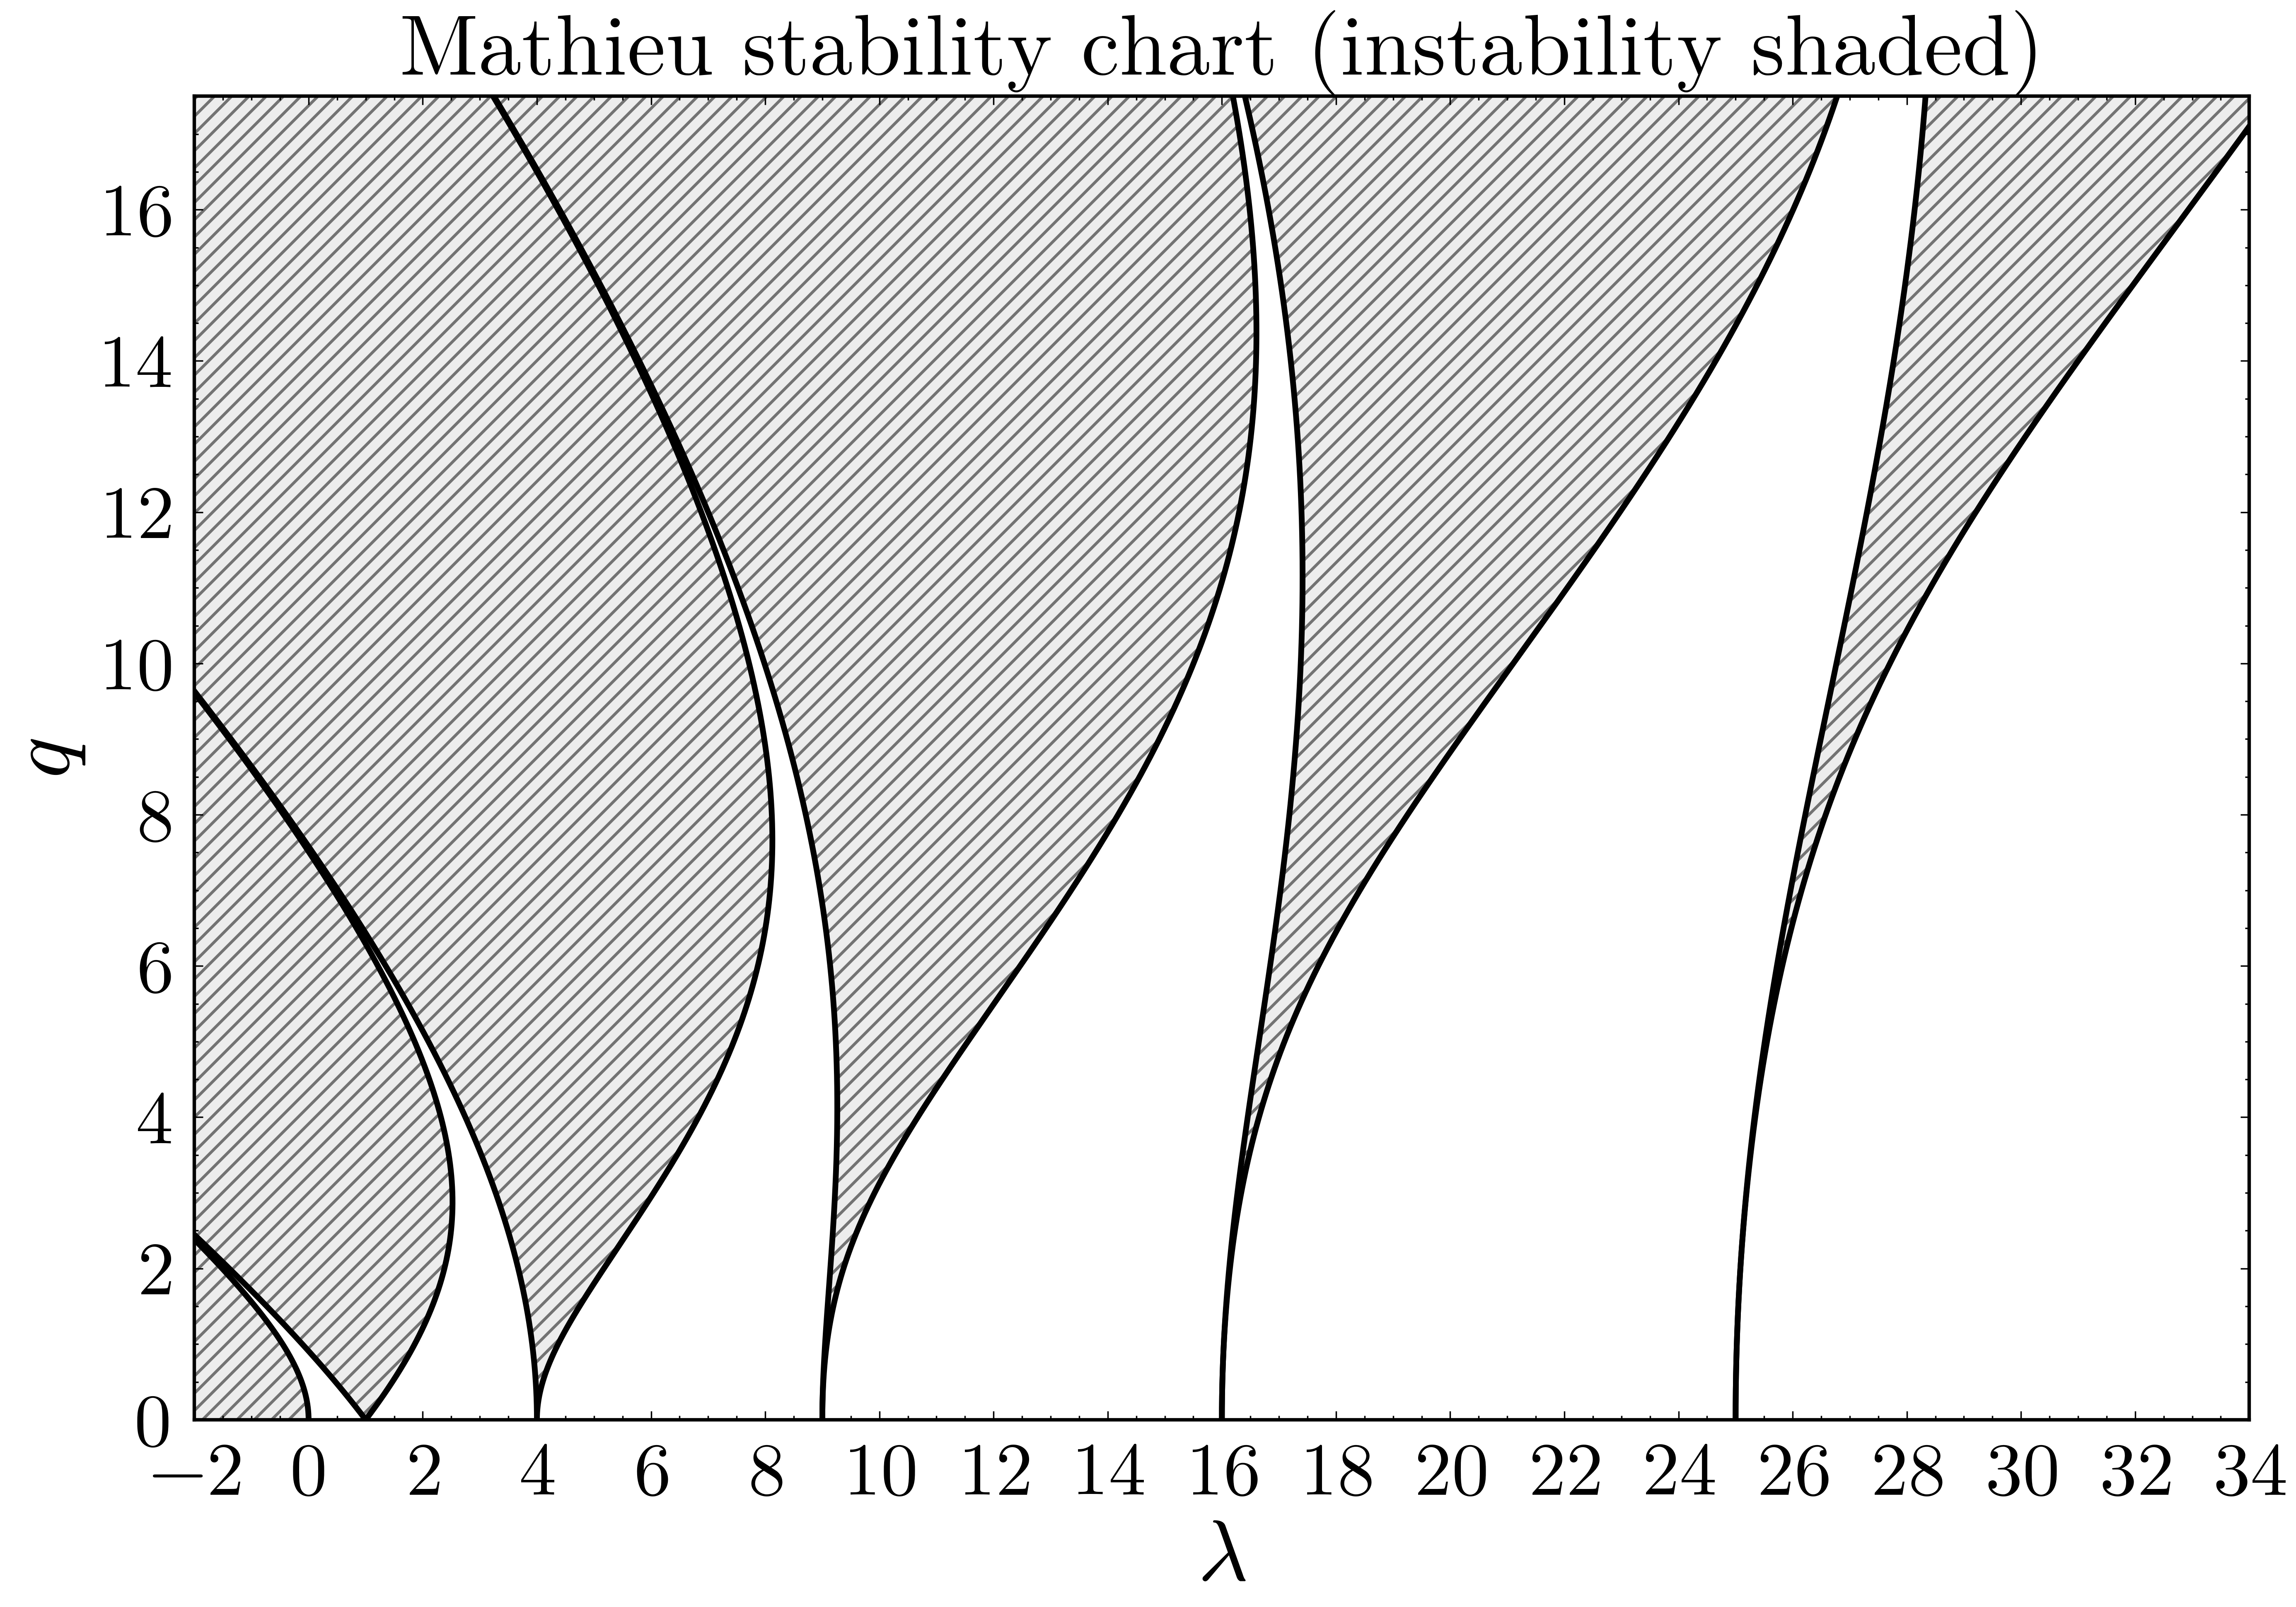
\includegraphics[width=\textwidth]{special_functions_fig/eigenvalue_curve_shaded_region_stable.png}
		\caption{本征值曲线（阴影区稳定）}
		\label{Mathieu方程解的示意图-本征值曲线(阴影区稳定)}
	\end{subfigure}
	\hfill
	\begin{subfigure}[b]{0.49\textwidth}
		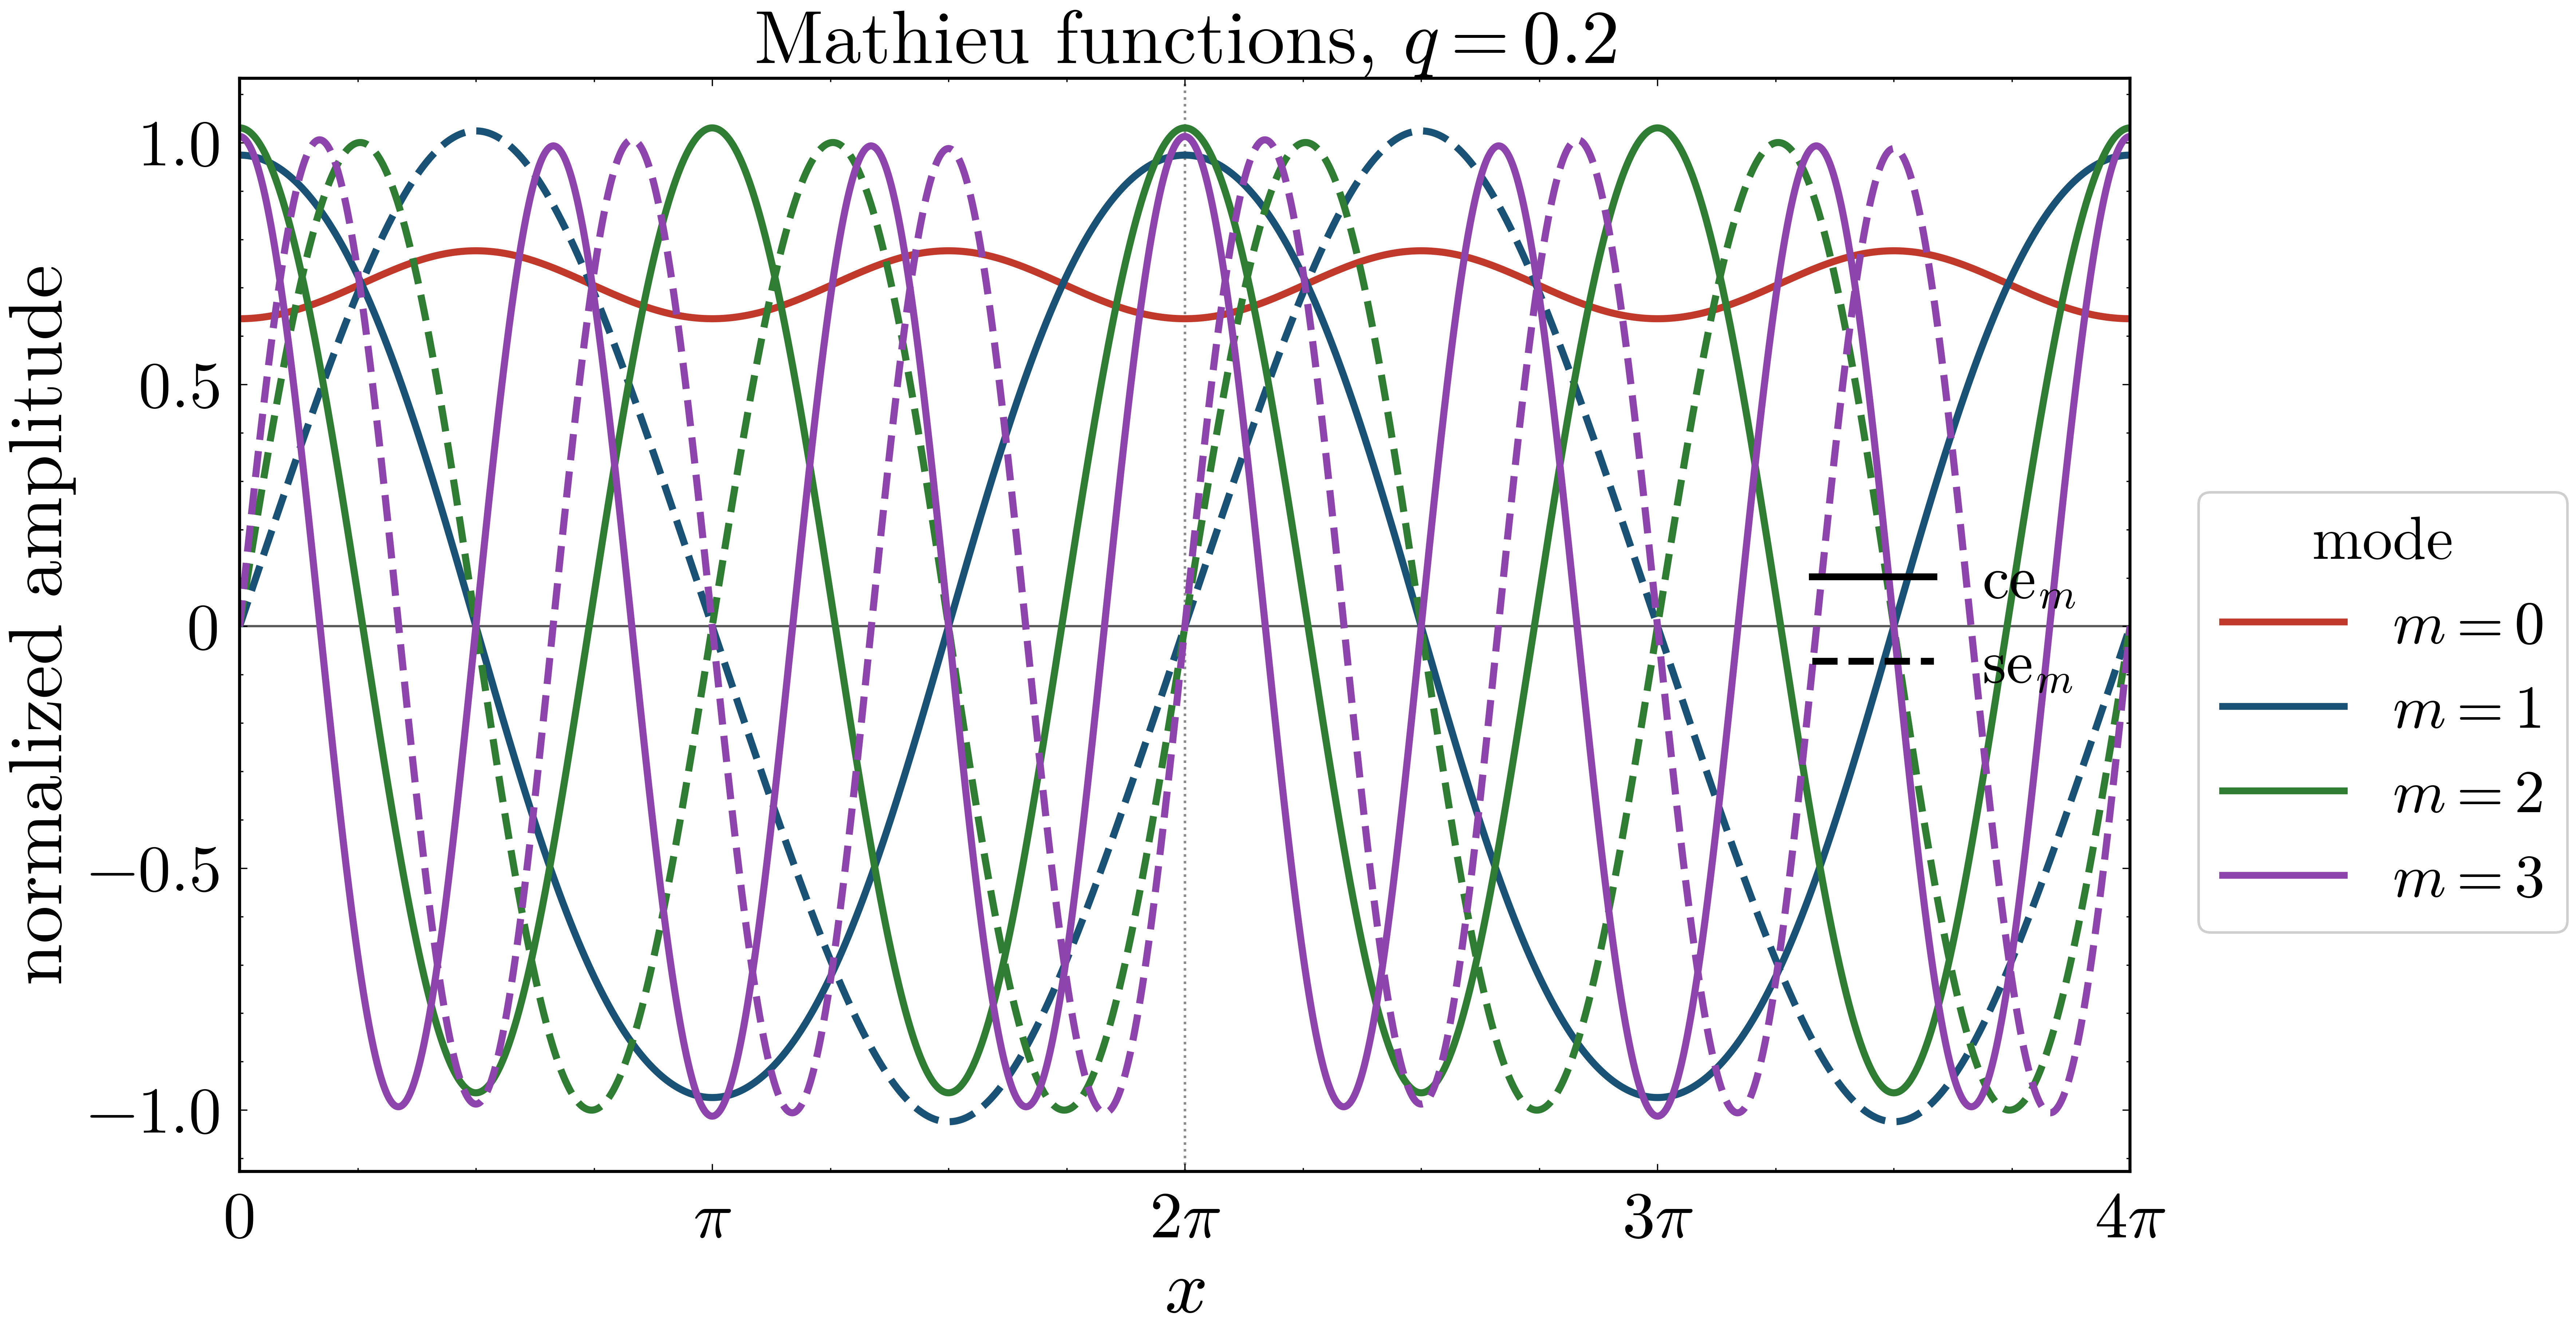
\includegraphics[width=\textwidth]{special_functions_fig/mathieu_function.png}
		\caption{Mathieu函数}
		\label{Mathieu方程解的示意图-Mathieu函数}
	\end{subfigure}
	\caption{Mathieu方程解的示意图}
	\label{Mathieu方程解的示意图}
\end{figure}

